\documentclass[crop=true,tikz,border=1pt,varwidth=8in]{standalone}

%\makeatletter
%%%%%%%%%%%%%%%%%
\PassOptionsToPackage{force}{filehook}
\usepackage{tikz}
\usetikzlibrary{shapes,arrows}
\usetikzlibrary{positioning}
\tikzstyle{cloud} = [draw, ellipse,fill=red!20, node distance=0.87cm,
minimum height=2em]
\tikzstyle{line} = [draw, -latex', color=yellow]
\usetikzlibrary{shapes.symbols,shapes.callouts,patterns}
\usetikzlibrary{calc}


\begin{document}
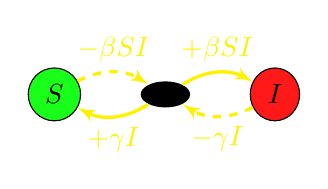
\begin{tikzpicture}[auto, %node distance = 2cm, auto,
	cloud/.style={minimum width={width("N-1")+2pt},
		draw, ellipse,fill=red!20}]
	\node[cloud, fill=green!90] (S) {$S$};
	\node[cloud, right=0.75cm of S, draw=none, fill=black] (h4) {};
	\node[cloud, right=0.75cm of h4, fill=red!90] (I) {$I$};
	%% Flows
	\path [line, bend left, very thick, dashed] (S) to node [midway, above] (TextNode) {$-\beta SI$} (h4);
	\path [line, bend left, very thick] (h4) to node [midway, below] (TextNode) {$+\gamma I$} (S);
	\path [line, bend left, very thick] (h4) to node [midway, above] (TextNode) {$+\beta SI$} (I);
	\path [line, bend left, very thick, dashed] (I) to node [midway, below] (TextNode) {$-\gamma I$} (h4);
\end{tikzpicture}
\end{document}